\section{Overview and Motivation (Discussion)}\label{sec:c9s1}
\lipsum[131-131]

This section builds on the material in \cref{ch:9}, \cref{ch:10} and the prior work of \citet{main-17}; see also \citep{main-27,main-38}.

\begin{equation}\label{eq:c9s1-a}
  I = \int_{0}^{1}\!\!\int_{0}^{1} \frac{\sin(\pi x)\sin(\pi y)}{1+x^2+y^2}\,\mathrm{d}x\,\mathrm{d}y \approx \frac{1}{M}\sum_{m=1}^{M} h(\xi_m),
\end{equation}
with variance decreasing as
\begin{equation}\label{eq:c9s1-b}
  \operatorname{Var}\bigl[\hat I_M\bigr] = \frac{1}{M}\Bigl(\int h^2\,\mathrm{d}\mu - I^2\Bigr) = \mathcal{O}(M^{-1}).
\end{equation}

Equations~\eqref{eq:c9s1-a} and~\eqref{eq:c9s1-b} are used throughout the remainder of this section.

\kant[4-11]

\subsection{Quantitative behaviour}\label{sec:c9s1-q}
Results are collected in \cref{tab:c9s1} and visualised in \cref{fig:c9s1-f1}. Similar trends were reported in~\citep{main-37,main-36}.

\begin{table}[htbp]
\centering
\caption{Summary of measured quantities for experiment set \texttt{c9s1}.}\label{tab:c9s1}
\begin{tabular}{lrrr}
\toprule
Method & Score & Latency & Error \\
\midrule
Alpha & \num{88.4} & \SI{6.56}{\milli\second} & \num{5.541e-3} \\
Beta & \num{81.9} & \SI{2.22}{\milli\second} & \num{3.779e-3} \\
Gamma & \num{6.8} & \SI{3.62}{\milli\second} & \num{8.844e-4} \\
Delta & \num{91.3} & \SI{6.55}{\milli\second} & \num{6.012e-2} \\
Epsilon & \num{5.1} & \SI{5.68}{\milli\second} & \num{5.637e-4} \\
\bottomrule
\end{tabular}
\end{table}

\begin{figure}[htbp]
\centering
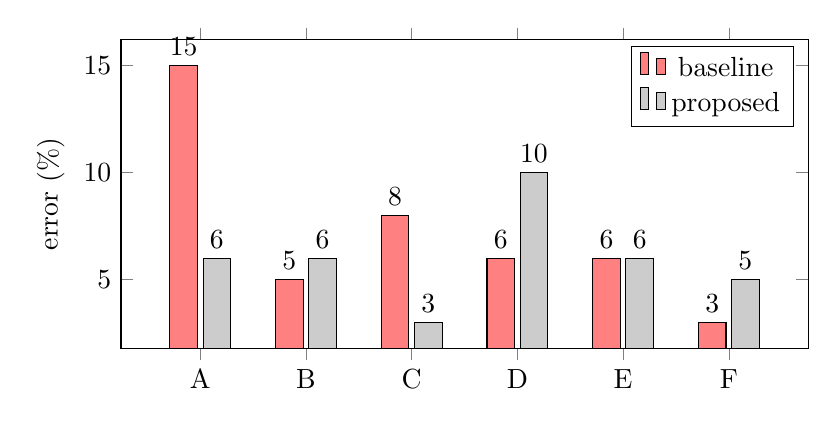
\begin{tikzpicture}\begin{axis}[ybar,width=0.85\linewidth,height=5.5cm,symbolic x coords={A,B,C,D,E,F},xtick=data,ylabel={error (\%)},enlarge x limits=0.15,bar width=10pt,nodes near coords]
\addplot[fill=red!50] coordinates {(A,15) (B,5) (C,8) (D,6) (E,6) (F,3)};
\addplot[fill=gray!40] coordinates {(A,6) (B,6) (C,3) (D,10) (E,6) (F,5)};
\legend{baseline,proposed}
\end{axis}\end{tikzpicture}
\caption{Generated figure for \texttt{c9s1-f1} (parameters $a=5$, $b=3$).}\label{fig:c9s1-f1}
\end{figure}

\kant[3-11]

\subsection{Implementation notes}\label{sec:c9s1-i}
The core routine is shown in \cref{lst:c9s1}; its complexity is $\mathcal{O}(N\log N)$ per iteration~\cite{main-21}.

\begin{lstlisting}[language=python,caption={Reference implementation for c9s1.},label={lst:c9s1}]
import numpy as np

def step(u, dt, dx, D):
    """Explicit finite-difference update."""
    lap = (np.roll(u, 1) - 2 * u + np.roll(u, -1)) / dx**2
    return u + dt * D * lap

u = np.exp(-((np.linspace(0, 1, 200) - 0.5) ** 2) / 0.01)
for _ in range(1000):
    u = step(u, 1e-5, 1 / 200, 1.0)
\end{lstlisting}

\kant[9-10]
\begin{theorem}\label{thm:c9s1}
Let $A\in\mathbb{R}^{n\times n}$ be symmetric positive definite with condition number $\kappa$. Then the iteration converges and
$\lVert e_k\rVert_A \le 2\bigl(\tfrac{\sqrt\kappa-1}{\sqrt\kappa+1}\bigr)^k\lVert e_0\rVert_A$.
\end{theorem}
\begin{enumerate}[label=(\roman*)]
\item the bound in \cref{thm:c9s1} is sharp for some initial errors;
\item the constant $2$ cannot be improved in general;
\item preconditioning reduces the effective $\kappa$.
\end{enumerate}

\begin{figure}[htbp]
\centering
\includegraphics[width=0.45\linewidth]{checker.png}
\caption{Raster/vector asset \texttt{checker.png} included from the figures directory.}\label{fig:c9s1-i0}
\end{figure}

\begin{figure}[htbp]
\centering
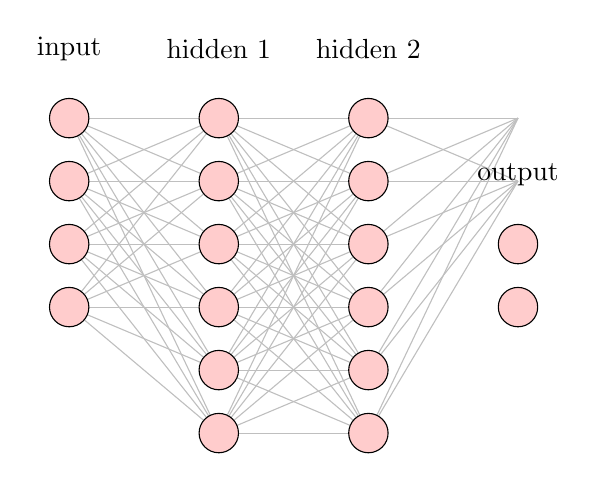
\begin{tikzpicture}[x=1.9cm,y=0.8cm,neuron/.style={circle,draw,fill=red!20,minimum size=5mm,inner sep=0}]
\foreach \i in {1,...,4}{\foreach \j in {1,...,6}{\draw[gray!50](0,-\i)--(1,-\j);}}
\foreach \i in {1,...,6}{\foreach \j in {1,...,6}{\draw[gray!50](1,-\i)--(2,-\j);}}
\foreach \i in {1,...,6}{\foreach \j in {1,...,2}{\draw[gray!50](2,-\i)--(3,-\j);}}
\foreach \i in {1,...,4}\node[neuron](i\i)at(0,-\i){};
\foreach \i in {1,...,6}\node[neuron](h\i)at(1,-\i){};
\foreach \i in {1,...,6}\node[neuron](g\i)at(2,-\i){};
\foreach \i in {1,...,2}\node[neuron](o\i)at(3,-\i-2){};
\node at(0,0.1){input};\node at(1,0.1){hidden 1};\node at(2,0.1){hidden 2};\node at(3,-1.9){output};
\end{tikzpicture}
\caption{Generated figure for \texttt{c9s1-f2} (parameters $a=2$, $b=6$).}\label{fig:c9s1-f2}
\end{figure}

\lipsum[119-119]
